\documentclass{article}

\usepackage{CJK}
\usepackage{graphicx}
\usepackage{amsmath}
\usepackage{color}
\usepackage{authblk}

\usepackage{geometry}
\usepackage{titlesec}


\addtolength{\topmargin}{-20pt}
\setlength{\oddsidemargin}{0.63cm}  % 3.17cm - 1 inch
\setlength{\evensidemargin}{\oddsidemargin}
\setlength{\textwidth}{14.66cm}
\setlength{\textheight}{22.00cm}    % 24.62

\linespread{1.5}
% \setlength{\parskip}{1ex}
\setlength{\parskip}{1\baselineskip}


\begin{document}


\title{\textbf{High-order Boltzmann Machine \\for Frame Ratio Upconversion}}
\author{Mingmin Zhao}
\affil{Department of Computer Science, Peking University, China}
%\author[*]{Author A}
%\author[*]{Author B}
%\author[*]{Author C}
%\author[**]{Author D}
%\author[**]{Author E}
%\affil[*]{Department of Computer Science, \LaTeX\ University}
%\affil[**]{Department of Mechanical Engineering, \LaTeX\ University}

\date{\today}
\maketitle
%\tableofcontents

%\newpage

\section{The model}

\begin{figure}
  \centering
  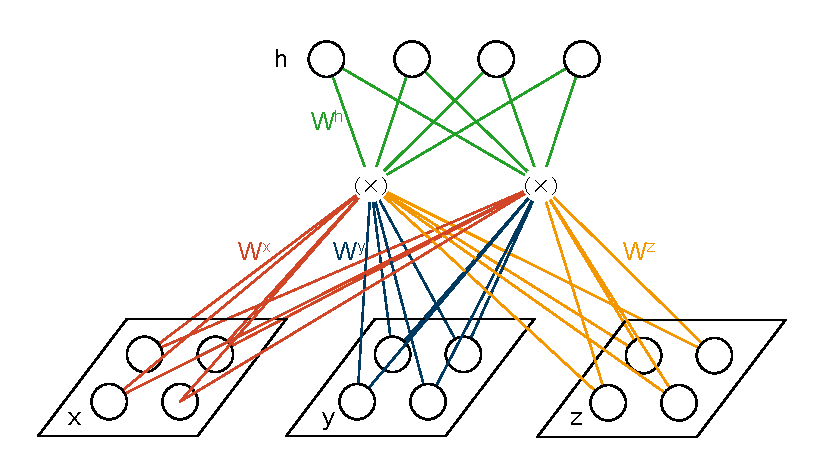
\includegraphics[width=3in]{4GRBM}\\
  \caption{Graphical representation of a 4-way Boltzmann machine}\label{4GRBM}
\end{figure}
sdfdsf


\subsection{High-order Boltzmann Machine}

\subsection{Learning}


\subsection{Inference}




\end{document}
